\section{Proces pomiarowy i~budowa zbioru danych} \label{sec:meas}
Zgodnie z~opisem technik termowizyjnych przedstawionym w~sekcji
\ref{sec:thermovision} zdecydowano się na przeprowadzenie pomiarów za pomocą
termowizji aktywnej.
Aby zrealizować pomiary uprzednio przygotowano stanowisko laboratoryjne.
Kamera termowizyjna została umieszczona na statywie, a~do ogrzewania próbek
zdecydowano się wykorzystać lampę halogenową.

W~procesie termowizji aktywnej istotna jest charakter procesu nagrzewania
materiału.
Przy przygotowaniu pomiarów należało zdecydować przy jakim warunku zakończyć
przekazywanie ciepła do próbki.
Rozważono dwie możliwości:
\begin{enumerate}[a)]
	\item ogrzewanie próbek do osiągnięcia ustalonej temperatury,
	\item \label{it:heatmethod} ogrzewanie próbek przez określony, stały czas.
\end{enumerate}
Zdecydowano się na metodę \ref{it:heatmethod}, ze względu na wygodę jej
realizacji.
Doprowadzenie każdej próbki do tej samej temperatury wymagałoby pomiarów
w~czasie nagrzewania, co jest bardziej wymagające do realizacji.
Zgodnie ze wstępnymi obserwacjami nagrzewanie materiału przez określony
czas pozwala na obserwację jego cech unikalnych i~wzorców zachowania podczas
stygnięcia.
Następnie należy wybrać czas nagrywania materiałów wideo kamerą.
Na podstawie wstępnych obserwacji i~próbnych nagrań zdecydowano się na
ogrzewanie próbek przez jedną minutę oraz rejestrację ich stygnięcia przez
cztery minuty.
Taka konfiguracja daje przy badanych pyłach rud miedzi ostry i~szczegółowy
obraz w~początkowej fazie nagrywania oraz widocznie rozmazany i~mniej
kontrastowy materiał pod koniec stygnięcia próbek.
Charakter procesu przejścia między tymi stanami pozwoli na klasyfikację
badanych próbek.
Ostatnia decyzja kształtująca charakter pomiarów dotyczy chwili
przechwytywania stopklatek z~pozyskanych materiałów wideo.
Na podstawie obserwacji zdecydowano się eksportować 5 klatek na początku
każdej minuty nagrania.
Po ustaleniu planu eksperymentu pomiarowego przystąpiono do jego wykonania.
Zgodnie z~opisem badanych materiałów w~sekcji \ref{sec:grains}, zgromadzono
materiały wideo dla czterech klas ziaren rudy miedzi.
Ze względu na czasochłonność pomiarów dla każdej klasy materiału nagrano trzy
materiały wideo.
Z~pozyskanych nagrań wyeksportowano stopklatki używając programu FLIR Tools,
pamiętając o~używaniu algorytmu automatycznego doboru zakresu temperatur
zgodnie z~opisem w~podsekcji \ref{subsec:camsoft}.

% TODO: Potem można tu wspomnieć że są wnioski na temat rozmiaru.

\section{Analiza zebranych obrazów termowizyjnych}
Zgodnie z~zamysłem pomiarów przedstawionym w~sekcji \ref{sec:meas} z~każdego
nagrania wybrano pięć stopklatek.
Podczas eksperymentu uzyskano łącznie dwanaście pomiarów, zawierających
sumarycznie 60 zdjęć.
W~ramach uczenia maszynowego jest to bardzo mały zbiór danych, biorąc jednak
pod uwagę wstępno-badawczy charakter pracy oraz czasochłonność procesu 
pomiarowego zdecydowano, że jest to rozmiar zadawalający do pierwszych
prób klasyfikacji.
% TODO: może przenieść do glosariusza
Zebrane materiały mają format JPEG, do oznaczania zdjęć przyjęto schemat
nazw jak w~przykładzie: 115\_E11R\_1, gdzie człony nazwy oznaczają kolejno:
\begin{itemize}
	\item automatyczny numer nagrania w~programie FLIR Tools,
	\item klasę próbki,
	\item minutę nagrania.
\end{itemize}

\subsection{Prezentacja przykładowej serii pomiarowej}
Jak opisano w rozdziale \ref{sec:meas} jedna próbka w~zbiorze danych 
składa się z~serii pięciu zdjęć o~malejącym kontraście i~szczegółowości.
Na rysunku \ref{fig:sample} przedstawiono przykładową próbkę 104 klasy E5R.
Widoczny jest proces stygnięcia materiału.
Skala po prawej stronie obrazów ma malejące na kolejnych obrazach wartości
co pokazuje że następuje zmniejszenie temperatury na całym obrazie.
Dodatkowo obraz staje się coraz mniej wyraźny i~kontrastowy.
Ze względu na budowę materiału nagrzana próbka emituje ciepłoze swoich
zróżnicowanych struktur w~niejednorodny sposób.
Wraz z~ochłodzeniem próbki jej temperatura się wyrównuje i~kamera termowizyjna
rejestruje coraz mniej szczegółów.
Detale i~elementy charakterystyczne obrazu zlewają się na kolejnych zdjęciach,
wraz z~opadaniem temperatury na zdjęciu pojawia się także coraz więcej szumów.
\begin{figure}[htbp]
	\centering
	\begin{subfigure}{0.45\textwidth}
		\centering
		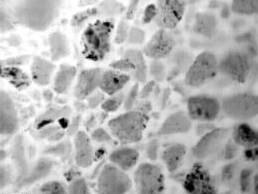
\includegraphics[width=\textwidth]{sample/104_E5R_0}
		\caption{Obraz z~próbki 104\_E5R\_0}
	\end{subfigure}
	\hspace{0.75cm}
	\vspace{0.5cm}
	\begin{subfigure}{0.45\textwidth}
		\centering
		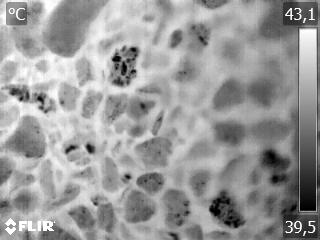
\includegraphics[width=\textwidth]{sample/104_E5R_1}
		\caption{Obraz z~próbki 104\_E5R\_1}
	\end{subfigure}
	\begin{subfigure}{0.45\textwidth}
		\centering
		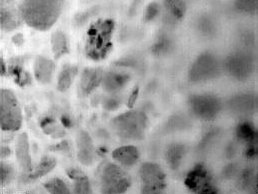
\includegraphics[width=\textwidth]{sample/104_E5R_2}
		\caption{Obraz z~próbki 104\_E5R\_2}
	\end{subfigure}
	\hspace{0.75cm}
	\vspace{0.5cm}
	\begin{subfigure}{0.45\textwidth}
		\centering
		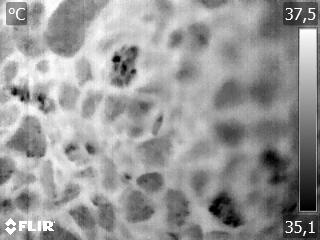
\includegraphics[width=\textwidth]{sample/104_E5R_3}
		\caption{Obraz z~próbki 104\_E5R\_3}
	\end{subfigure}
	\begin{subfigure}{0.45\textwidth}
		\centering
		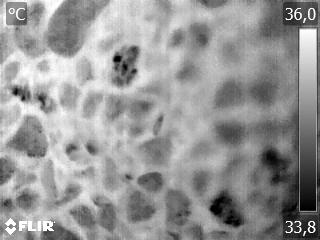
\includegraphics[width=\textwidth]{sample/104_E5R_4}
		\caption{Obraz z~próbki 104\_E5R\_4}
	\end{subfigure}
	\caption{Zdjęcia procesu stygnięcia w~przykładowej próbce 104 klasy E5R}
	\label{fig:sample}
\end{figure}

\subsection{Przetwarzanie danych wizyjnych}

\subsection{Poprawa jakości obrazu}

\subsection{Automatyczny odczyt zakresu pomiarowego temperatur z~obrazu}
Jak wspomniano w~sekcji \ref{subsec:camsoft} jednym z~kluczowych czynników
decydujących o~wyglądzie obrazów pochodzących z~kamery jest zakres temperatur
mapowany na kolory w~obrazie.
Niestety aplikacja FLIR Tools nie pozwala na eksport zakresu temperatur wraz
ze zdjęciami w~formie liczbowej.
W~czasie zapisu zdjęć oprogramowanie dodaje na nich interfejs z~aktywną skalą
pomiarową, jednak jest on graficznie naniesiony na obraz.
Aby ułatwić w przyszłości pracę z~materiałami z~kamery opracowano dodatkowo
mechanizm ekstrakcji zakresu temperatur z~zdjęć pochodzących z kamery.

W~celu konstrukcji funkcji odczytu wartości liczbowych z~obrazu posłużono
się gotową siecią neuronową zaprojektowaną do detekcji tekstu na zdjęciach.
Zdecydowano się na użycie popularnej biblioteki \emph{Pytesseract}.
Aby poprawnie odczytać wartości z~obrazu najpierw przycięto je tak by w~kadrze
znajdowała się tylko odczytywana liczba.
Ponieważ przy eksporcie zdjęć program FLIR Tools nakłada interfejs na zdjęcia
w~identyczny sposób, kadrowanie obrazu jest takie same dla każdej próbki
pomiarowej.
Wycięte kadry są bardzo małej rozdzielczości, aby ułatwić sieci rozpoznawanie
liczb zdecydowano się przeskalować je w~górę.
W~czasie skalowania włączono mechanizm anty aliasingu aby wyrównać krawędzie
cyfr.
Ponieważ używana sieć uznaje za tło kolor biały oraz poszukuje liczb w~kolorze
czarnym barwy na zdjęciu odwrócono.
Następnie obraz poddano binaryzacji metodą \emph{otsu}.
Jest to popularna i~wydajna metoda binaryzacji, jej efektywność jest
maksymalna kiedy ilość pikseli tła oraz pierwszego planu jest zbliżona,
dlatego poprawne kadrowanie liczb sprzyja jakości ich binaryzacji\cite{sezgin}.
Na rysunku \ref{fig:temp_bounds} przedstawiono kolejne etapy przygotowania
obrazu do rozpoznania liczb.
Implementację opisanego mechanizmu odczytywania zakresu temperatur ze zdjęć
przedstawiono na listingu \ref{lst:temp_bounds}.
\begin{figure}[htbp]
	\centering
	\begin{subfigure}{0.45\textwidth}
		\centering
		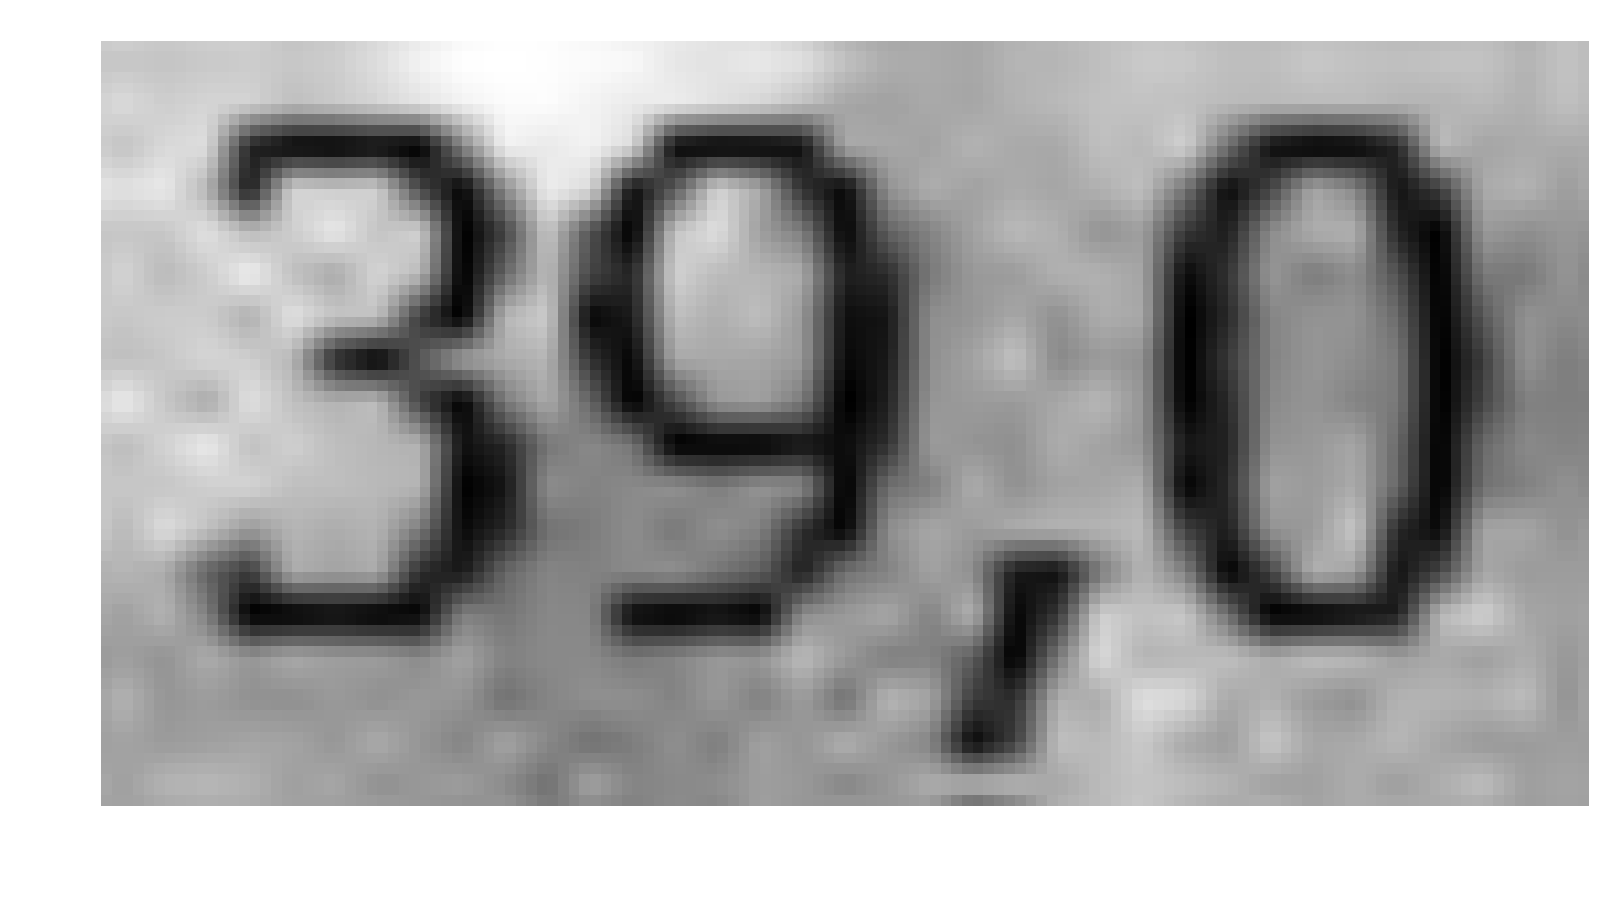
\includegraphics[width=\textwidth]{temp_bounds_scale}
		\caption{Przeskalowany kadr z~liczbą}
		\label{fig:temp_bounds_scale}
	\end{subfigure}
	\hspace{0.5cm}
	\begin{subfigure}{0.45\textwidth}
		\centering
		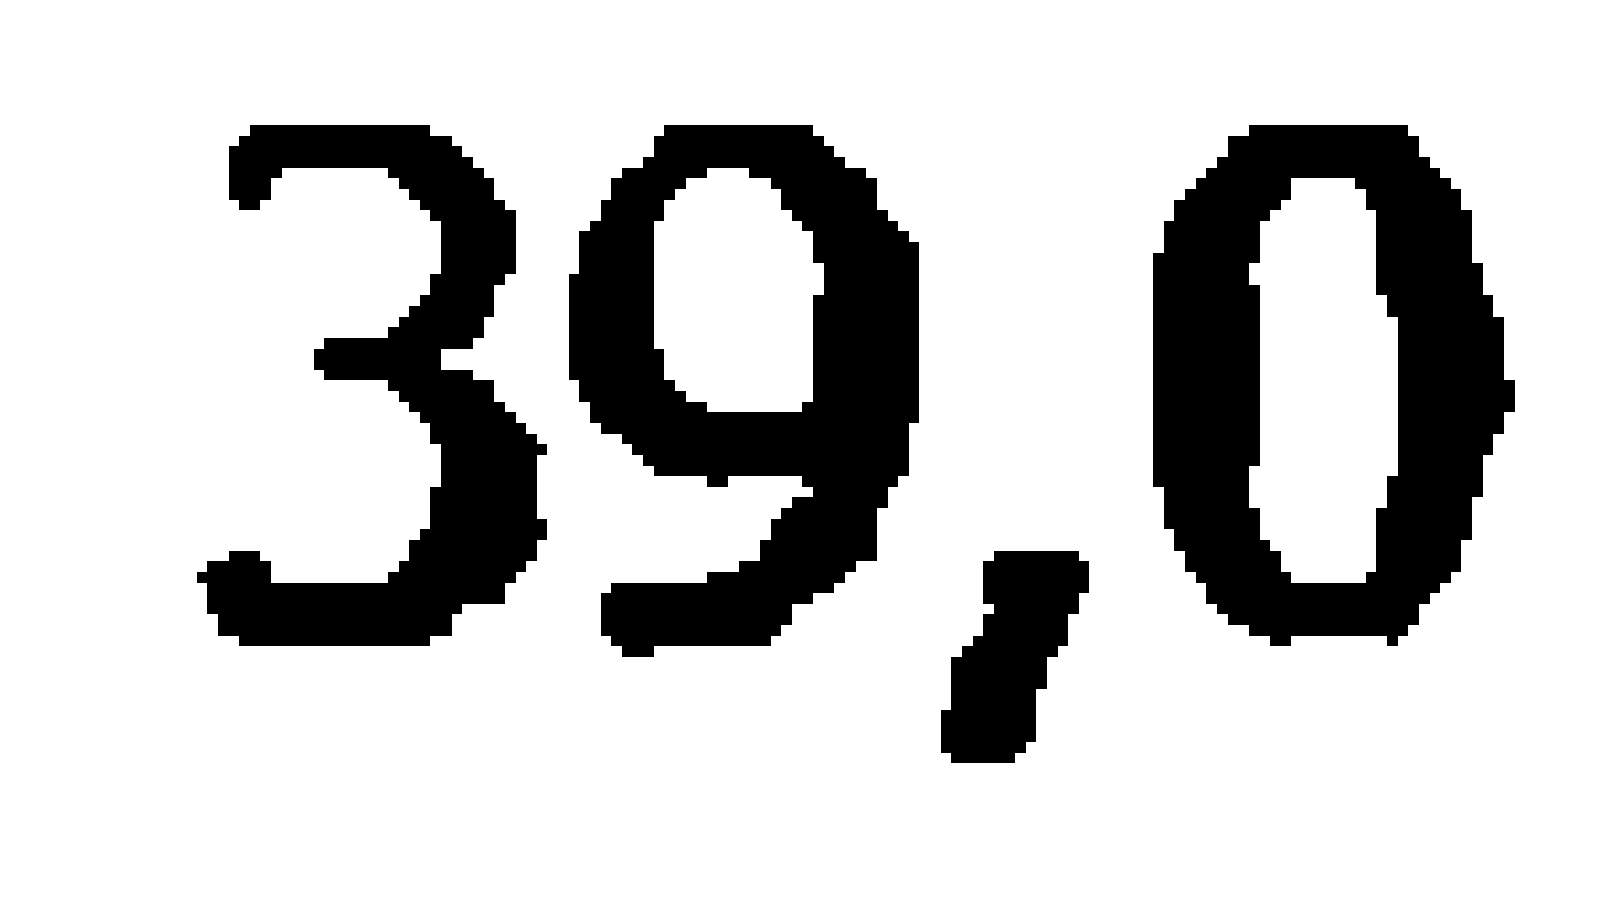
\includegraphics[width=\textwidth]{temp_bounds_bin}
		\caption{Kadr z~liczbą po binaryzacji}
		\label{fig:temp_bounds_bin}
	\end{subfigure}
	\caption{Przygotowanie zakresu temperatur do odczytu przez sieć neuronową}
	\label{fig:temp_bounds}
\end{figure}

% TODO: This code might be not ready
\begin{listing}[htbp]
\begin{minted}{python}
def get_temperature_bounds(img, bounds=(((6, 24), (283, 318)),
                                       ((219, 236), (283, 318)))):
    '''Extract temperature values from FLIR UI on image.'''
    img = invert(img)
    temp_txt = []
    for bound in bounds:
        bound_img = img[slice(*bound[0]), slice(*bound[1])]
        bound_img = rescale(bound_img, 4, anti_aliasing=True)
        thr = threshold_otsu(bound_img)
        img_txt = bound_img > thr
        img_txt = Image.fromarray(img_txt)
        temp = pytesseract.image_to_string(img_txt)
        if temp is not '': 
            temp = float(temp)
        else:
            temp = 0
        temp_txt.append(temp)
    return temp_txt
\end{minted}
\caption{Funkcja języka Python do odczytywania zakresu temperatur ze zdjęć
         z~kamery}
\label{lst:temp_bounds}
\end{listing}

\section{Poszukiwanie zależności użytecznych w~klasyfikacji}
Aby móc klasyfikować dane należy zastanowić się nad cechami które je
odróżniają.
Na rysunku \ref{fig:samplecompare} przedstawiono porównanie stygnięcia
dwóch rodzajów próbek: E5R oraz E6R.
W~klasyfikacji użyteczne będą dane które są unikalne dla danej klasy.
Ponieważ dane stanowią serię obrazów postępującego studzenia materiału, aby
wykorzystać pełnię możliwości zebranych zdjęć warto szukać cech
charakterystycznych dla przebiegu procesu chłodzenia.
\begin{figure}[htbp]
	\centering
	\begin{subfigure}{0.3\textwidth}
		\centering
		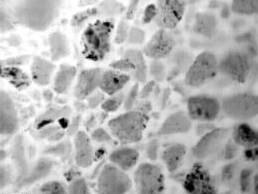
\includegraphics[width=\textwidth]{sample/104_E5R_0}
		\caption{Próbka 104\_E5R\_0}
	\end{subfigure}
	\hspace{0.25cm}
	\vspace{0.5cm}
	\begin{subfigure}{0.3\textwidth}
		\centering
		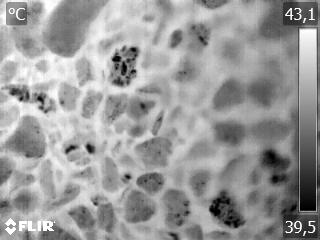
\includegraphics[width=\textwidth]{sample/104_E5R_1}
		\caption{Próbka 104\_E5R\_1}
	\end{subfigure}
	\hspace{0.25cm}
	\begin{subfigure}{0.3\textwidth}
		\centering
		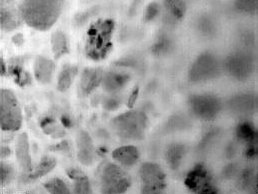
\includegraphics[width=\textwidth]{sample/104_E5R_2}
		\caption{Próbka 104\_E5R\_2}
	\end{subfigure}
	\begin{subfigure}{0.3\textwidth}
		\centering
		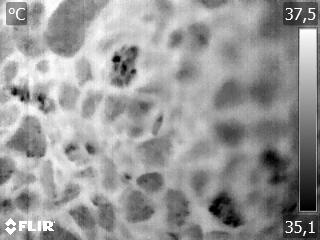
\includegraphics[width=\textwidth]{sample/104_E5R_3}
		\caption{Próbka 104\_E5R\_3}
	\end{subfigure}
	\hspace{0.25cm}
	\vspace{0.5cm}
	\begin{subfigure}{0.3\textwidth}
		\centering
		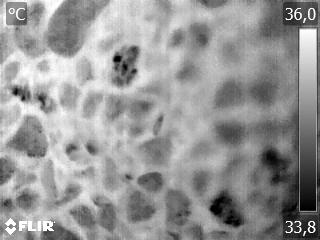
\includegraphics[width=\textwidth]{sample/104_E5R_4}
		\caption{Próbka 104\_E5R\_4}
	\end{subfigure}
	\hspace{0.25cm}
	\begin{subfigure}{0.3\textwidth}
		\centering
		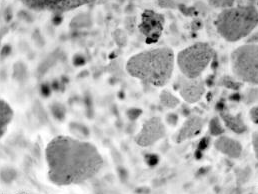
\includegraphics[width=\textwidth]{sample/117_E6R_0}
		\caption{Próbka 117\_E6R\_0}
	\end{subfigure}
	\begin{subfigure}{0.3\textwidth}
		\centering
		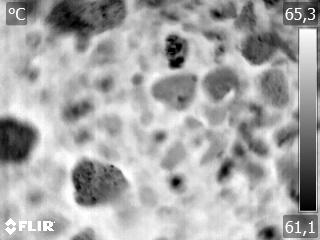
\includegraphics[width=\textwidth]{sample/117_E6R_1}
		\caption{Próbka 117\_E6R\_1}
	\end{subfigure}
	\hspace{0.25cm}
	\vspace{0.5cm}
	\begin{subfigure}{0.3\textwidth}
		\centering
		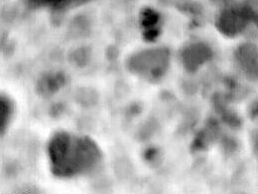
\includegraphics[width=\textwidth]{sample/117_E6R_2}
		\caption{Próbka 117\_E6R\_2}
	\end{subfigure}
	\hspace{0.25cm}
	\begin{subfigure}{0.3\textwidth}
		\centering
		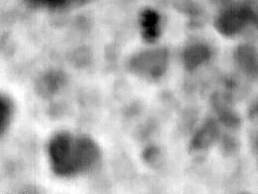
\includegraphics[width=\textwidth]{sample/117_E6R_3}
		\caption{Próbka 117\_E6R\_3}
	\end{subfigure}
	\begin{subfigure}{0.3\textwidth}
		\centering
		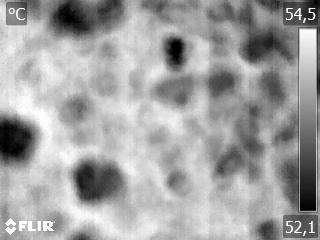
\includegraphics[width=\textwidth]{sample/117_E6R_4}
		\caption{Próbka 117\_E6R\_4}
	\end{subfigure}
	\caption{Porównanie procesu stygnięcia próbek klasy E5R oraz E6R}
	\label{fig:samplecompare}
\end{figure}

\subsection{Wybór cech obrazu użytecznych w~klasyfikacji}
\label{subsec:featureextr}
Po przyjrzeniu się rysunkowi \ref{fig:samplecompare} widoczne  jest, że
w~próbce E6R temperatura ziaren zaczęła wyrównywać się szybciej.
Na podstawie obserwacji zebranych danych rozpatrzono następujące możliwości
obserwacji cech charakterystycznych materiałów:
\begin{enumerate}[a)]
	\item \label{it:imgcnn} 
	      klasyfikacja zdjęć w~całości jako macierzy danych przez złożoną sieć
	      konwolucyjną,
	\item \label{it:fft} 
	      analiza częstotliwościowa obrazów w~celu śledzenia tempa rozmycia
	      kolejnych zdjęć,
	\item \label{it:glcm} 
	      użycie macierzy GLCM jako wejścia sieci neuronowych,
	\item \label{it:edge}
	      wykrywanie krawędzi ziaren i~wyznaczanie reprezentacji liczbowej
	      ich kształtów oraz powierzchni,
	\item \label{it:blob}
	      śledzenie zlewania się i~zanikania małych detali na obrazie.
\end{enumerate}

Wszystkie przedstawione opcje mają uzasadnienie i~mogą sprawdzić się dobrze
jako podstawa klasyfikacji.
Należy jednak ocenić której z~nich użyć w~pierwszej próbie konstrukcji
klasyfikatora. Metoda \ref{it:imgcnn}, z~użyciem sieci konwolucyjnych może
wykorzystywać najnowsze rozwiązania w~dziecinie uczenia maszynowego,
jednak przy jej użyciu na przeszkodzie może stać bardzo mały rozmiar zbioru
uczącego.
Na niewielu zgromadzonych obrazach znajduje się wiele informacji i~szumów,
a~złożoność jednego zdjęcia jest na tę chwilę nieproporcjonalna do wielkości
zbioru danych.
Pomysł ten można spróbować zrealizować po rozszerzeniu pomiarów.
Kolejna opcja \ref{it:fft} z~użyciem analizy częstotliwościowej wymaga
złożonych operacji matematycznych i~może być wrażliwa na szumu na obrazie.
Po analizie innych opcji zdecydowano, że istnieją bardziej obiecujące
alternatywy.
Macierz glcm (\textit{Gray-Level Co-Occurrence Matrix}), na której może
bazować opcja \ref{it:glcm}, to tablica zawierająca informacje o~relacjach
wszystkich par pikseli na obrazie.
Pozwala ona na analizę takich wartości jak: kontrast, korelacja, energia
oraz homogeniczność.
Jest to opcja dająca możliwość analizy dużej ilości informacji, z~pewnością
warta rozpatrzenia, jednak dosyć skomplikowana.
Na obrazie można także wykrywać kształty ziaren za pomocą filtrów detekcji
krawędzi.
Opcję tę testowano przy pomocy filtra \emph{Canny}.
Krawędzie ziaren okazały się jedank trudne do wykrycia kształtów i~dalszej
segmentacji ze względu na małą rodzielczość oraz duże upakowanie ziaren.
Operacje morfologiczne domykania kształtów powodowały bardzo duże zmiany
w~obrazie i~zlewały ziarna.
Rozwój takiego podejścia przy analizowanych obrazach wymaga zaawansowanej
i~ostrożnej obróbki zdjęć.
Ostatnia opcja \ref{it:blob} wynika z~obserwacji detali na obrazach.
Na przedstawionych zdjęciach próbek można zauważyć drobne ciemne punkty,
które są obszarami o~wolniejszej wymianie ciepła z~otoczeniem niż reszta
powierzchni ziaren.
Na rysunku \ref{fig:blobdetail} przedstawiono zbliżenie na grupę takich
detali, w~czterech częściach procesu stygnięcia.
\begin{figure}[htbp]
	\centering
	\begin{subfigure}{0.3\textwidth}
		\centering
		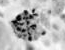
\includegraphics[width=\textwidth]{sample/detail_119_E5R_0}
		\caption{Grupa detali w~próbce 119\_E5R\_0}
	\end{subfigure}
	\hspace{0.25cm}
	\centering
	\begin{subfigure}{0.3\textwidth}
		\centering
		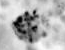
\includegraphics[width=\textwidth]{sample/detail_119_E5R_1}
		\caption{Grupa detali w~próbce 119\_E5R\_1}
	\end{subfigure}
	\hspace{0.24cm}
	\begin{subfigure}{0.3\textwidth}
		\centering
		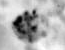
\includegraphics[width=\textwidth]{sample/detail_119_E5R_2}
		\caption{Grupa detali w~próbce 119\_E5R\_2}
	\end{subfigure}
	\caption{Zbliżenie na charakterystyczne grupy detali materiału}
	\label{fig:blobdetail}
\end{figure}
Analizując próbki można zauważyć, że wraz ze stygnięciem ciemne punkty
w~grupach zlewają się, a~następnie zanikają.
Dodatkowo ich liczba na poszczególnych klasach materiałów jest różna.
Zdecydowano się na wybór metody polegającej na śledzeniu liczby tych punktów
i~ich zaniku.
Taka analiza wiąże się z~przetwarzaniem obrazów i~utworzeniem algorytmów
śledzenia detali.
Opcja ta wydaje się jednak obiecująca, ponieważ nawet podczas wstępnej
obserwacji próbek można dopatrywać się zależności miedzy klasami a~obecnością
omawianych detali.

\subsection{Wybór algorytmu detekcji ziaren}
Zgodnie z~rozważaniami przedstawionymi w~podsekcji \ref{subsec:featureextr}
w celu klasyfikacji ziaren zdecydowano się na obserwację ilości ciemnych,
drobnych detali na obrazach.
Należy więc wybrać metodę detekcji charakterystycznych punktów.
W~wykrywaniu omawianych detali użyteczne są algorytmy wykrywania plam na
podstawie analizy pochodnych wartości na obrazie.
Biblioteka Scikit-image udostępnia trzy algorytmy tego typu wykorzystujące:
\begin{enumerate}[a)]
	\item laplasjan funkcji Gaussa,
	\item różnica funkcji Gaussa,
	\item wyznacznik Hesjanu.
\end{enumerate}

Metoda bazująca na laplasjanie funkcji Gaussa jest najdokładniejsza, ale
także najwolniejsza.
Funkcja Gaussa, której wykres ma charakterystyczny kształt krzywej dzwonowej
jest dana wzorem \ref{eq:gaussian}, gdzie:
\begin{itemize}
	\item $ \sigma $ to odchylenie standardowe,
	\item $ \mu $ to wartość średnia.
\end{itemize}
\begin{equation}
	P(x) = \frac{1}{{\sigma \sqrt {2\pi } }}
	e^{{{ - \left( {x - \mu } \right)^2 }
	\mathord{\left/ {\vphantom {{ - \left( {x - \mu } \right)^2 }
	{2\sigma ^2 }}} \right. \kern-\nulldelimiterspace} {2\sigma ^2 }}}
\label{eq:gaussian}
\end{equation}
Laplasjan to operator różniczkowy drugiego rzędu.
Omawiany algorytm oblicza wartości funkcji Gaussa dla coraz większego
odchylenia standardowego i~układa je w~sześcianie.
Poszukiwane plamy to lokalne maksima w~tym sześcianie.
Wadą tego rozwiązania jest bardzo wolne wykrywanie dużych plam z~powodu
złożoności obliczeniowej.

Różnica funkcji Gaussa jest metodą podobną do poprzedniej.
Ponownie rozmywa ona obrazu z~narastającymi odchyleniami standardowymi
z~użyciem funkcji Gaussa.
Następnie różnice rozmytych obrazów są układane w~sześcianie, gdzie
maksima to plamy.
Metoda ta jest szybsza i~mniej dokładna od algorytmu bazującego na laplasjanie
funkcji Gaussa, ale podobnie jak ona jest wolna w wykrywaniu dużych elementów.

Ostatnia metoda jest najszybsza, ale najmniej dokładna.
Polega ona na wyszukiwaniu maksimów w~macierzy Hesjanu, jest to macierz
drugich pochodnych cząstkowych.
Postać takiej macierzy w~n-wymiarowej przestrzeni przedstawia wzór
\ref{eq:hessian}.
Prędkość tej metody nie zależy od wielkości wykrywanych plam, ale małe
elementy mogą nie zostać przez nią wykryte.
\begin{equation}
	H = \begin{bmatrix}
	\dfrac{\partial^2 f}{\partial x_1^2} & 
	\dfrac{\partial^2 f}{\partial x_1\,\partial x_2} & 
	\cdots & \dfrac{\partial^2 f}{\partial x_1\,\partial x_n} \\[2.2ex]
	\dfrac{\partial^2 f}{\partial x_2\,\partial x_1} &
	\dfrac{\partial^2 f}{\partial x_2^2} &
	\cdots & \dfrac{\partial^2 f}{\partial x_2\,\partial x_n} \\[2.2ex]
	\vdots & \vdots & \ddots & \vdots \\[2.2ex]
	\dfrac{\partial^2 f}{\partial x_n\,\partial x_1} &
	\dfrac{\partial^2 f}{\partial x_n\,\partial x_2} &
	\cdots &
	\dfrac{\partial^2 f}{\partial x_n^2}
	\end{bmatrix}
\label{eq:hessian}
\end{equation}

Porównanie działania wymienionych metod przedstawiono na grafice
\ref{fig:blobcompare}.
Jak można było spodziewać się po opisie funkcji najlepsza okazała się metoda
Laplasjanu funkcji Gaussa.
Funkcję korzystającą z~wyznacznika Hesjanu należy odrzucić, ponieważ
w~rozważanym przypadku istotne jest wykrywanie małych plam.
Z~tego samego powodu korzystne jest użycie najbardziej dokładnej funkcji.
Ponieważ program nie ma wykrywać dużych elementów nie ma ryzyka zbyt
powolnych obliczeń na obszernych plamach.

\begin{figure}[htbp]
	\centering
	\begin{subfigure}[t]{0.3\textwidth}
		\centering
		\includegraphics[width=\textwidth]{example-image}
		\caption{Laplasjan funkcji Gaussa}
	\end{subfigure}
	\hspace{0.25cm}
	\centering
	\begin{subfigure}[t]{0.3\textwidth}
		\centering
		\includegraphics[width=\textwidth]{example-image}
		\caption{Różnica funkcji Gaussa}
	\end{subfigure}
	\hspace{0.25cm}
	\begin{subfigure}[t]{0.3\textwidth}
		\centering
		\includegraphics[width=\textwidth]{example-image}
		\caption{Wyznacznik Hesjanu}
	\end{subfigure}
	\caption{Porównanie bibliotecznych algorytmów wykrywania plam w~obrazie}
	\label{fig:blobcompare}
\end{figure}

Aby wybrana funkcja laplasjanu funkcji Gaussa wykrywała, zgodnie
zamierzeniami tylko małe plamy należy podać jej odpowiednie parametry,
co uczyniono już na etapie porównania metod detekcji.
Wywołanie omawianej funkcji ma postać:
\mintinline{python}{blobs = blob_dog(img, max_sigma=2, threshold=0.1)}.
Funkcji podano dwa dodatkowe argumenty, które są istotne dla pożądanego
działania.
Argument \mintinline{python}{max_sigma=2} ogranicza odchylenie standardowe
obliczanych funkcji Gaussa, przez co wykrywane są tylko małe elementy.
Drugi argument \mintinline{python}{threshold=0.1} decyduje o~poziomie
powyżej jakiego punkt jest uznany za maksimum w~sześcianie laplasjanów.
Domyślna wartość tego argumentu \mintinline{python}{threshold=2.0} okazała 
się za duża, zmniejszono jej wartość aby wykrywać bardziej subtelne detale.
Na podstawie opisanego wywołania metody Laplasjanu funkcji Gaussa
opracowano funkcję zwracającą położenie i~promienie wykrytych plam.

\subsection{Algorytm śledzenia ziaren w~serii zdjęć}

\subsection{Wizualizacja zebranych cech i~ocena ich użyteczności}
